\section[Desenvolvimento do Projeto]{Desenvolvimento do Projeto}
Ao longo desta seção, são apresentados os artefatos desenvolvidos ao longo do
semestre no qual se situou o projeto. Também estão descritas as etapas realizadas
para as entregas destes artefatos, bem como ilustrações e seus respectivos para a \textit{wiki} do projeto.

\subsection{Repositório do Código Fonte do Projeto}
O projeto foi estruturado em três repositórios distintos, cada um abrigando artefatos específicos. O repositório "Wiki"~incluía toda a documentação de arquitetura e requisitos, além de materiais para estudos dirigidos e os protótipos de telas.

Além da \textit{wiki}, foram criados os repositórios "soul-amada-backend"~e "soul-amada-frontend"~para guardar o código do projeto. Todos estes podem ser encontrados no link: \url{https://tools.ages.pucrs.br/soul-amada}.

\subsection{Banco de Dados Utilizado}
Diante dos requisitos simples para a persistência dos dados, optou-se por utilizar um banco relacional. A ideia inicial era tão simples que, em um primeiro momento, foram conceitualizadas apenas duas tabelas, conforme a figura 13.

\begin{figure}[H]
  \centering
  \small
  \caption{Diagrama conceitual inicial do banco de dados do projeto Soul Amada}
  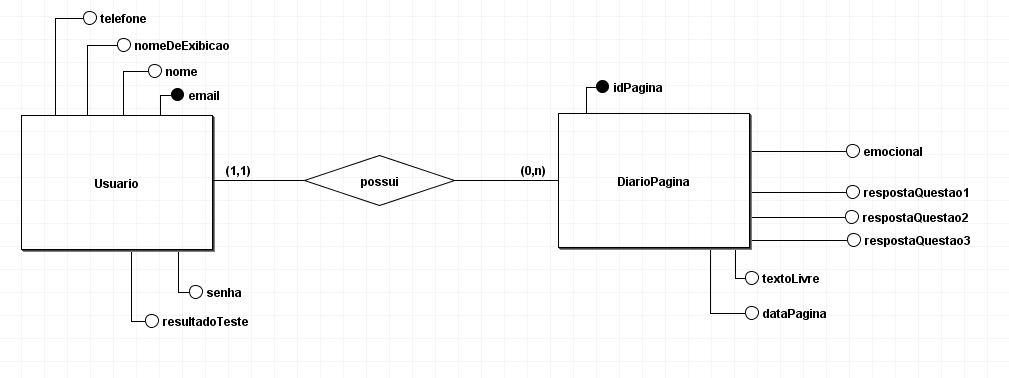
\includegraphics[width=1\linewidth]{conteudo//3 - ages II//conteudo//figures/soul-bd-concept}
  Fonte: \textit{Wiki} do projeto
  \label{fig:db-concept}
\end{figure}

O intuito era de que o banco de dados fosse simples e contivesse apenas tabelas para os usuários e outra para as postagens. Os dados adicionais que não precisariam de tabelas (devocionais e vídeo aulas) iriam ser armazenados diretamente no código do \textit{frontend}.

No entanto, notou-se que estes dados ou poderiam ser alterados com frequência ou eram muito extensos, o que poderia causar dores de cabeça futuras. Por isso, froam criadas tabelas para estes dados também.

Em um processo iterativo com nossos AGES IV e AGES III, o modelo do banco passou por alterações e atualizações à medida que as primeiras \textit{sprints} foram ocorrendo. Os diagramas finais, tanto o conceitual quanto o lógico, estão ilustrados nas figuras 14 e 15, respectivamente.

\begin{figure}[H]
  \centering
  \small
  \caption{Diagrama conceitual final do banco de dados do projeto Soul Amada}
  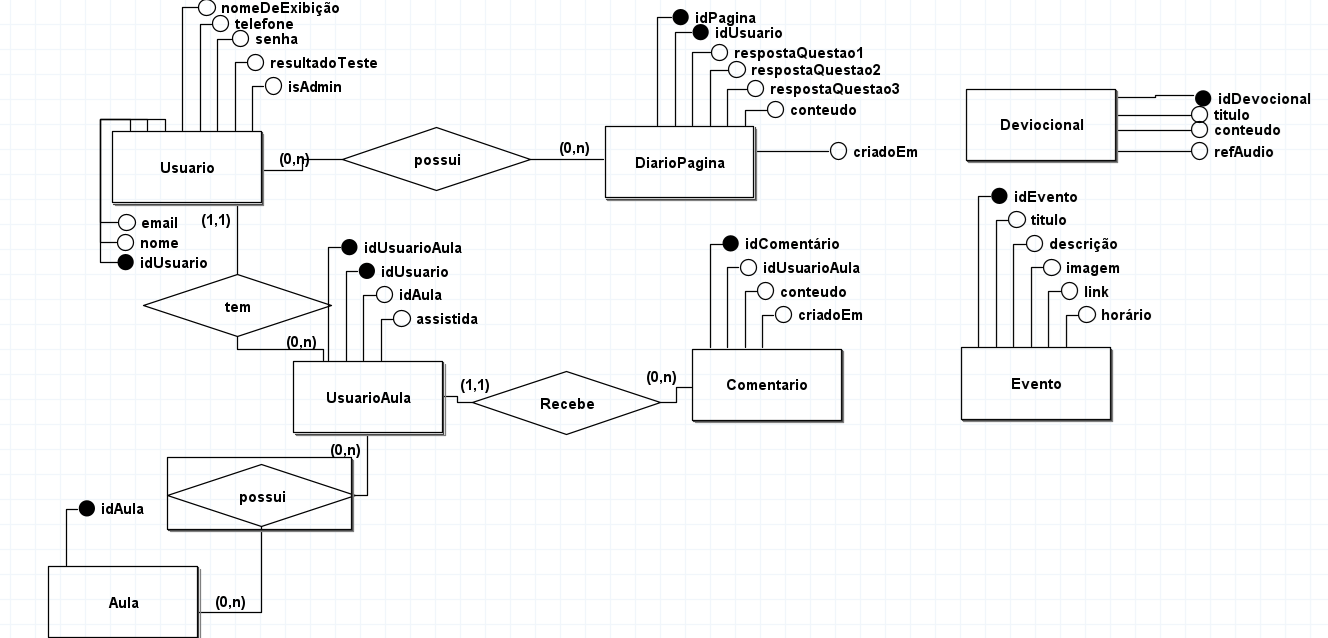
\includegraphics[width=1\linewidth]{conteudo//3 - ages II//conteudo//figures/soul-bd-concept2}
  Fonte: \textit{Wiki} do projeto
  \label{fig:db-concept2}
\end{figure}

\begin{figure}[H]
  \centering
  \small
  \caption{Diagrama lógico do banco de dados do projeto Soul Amada}
  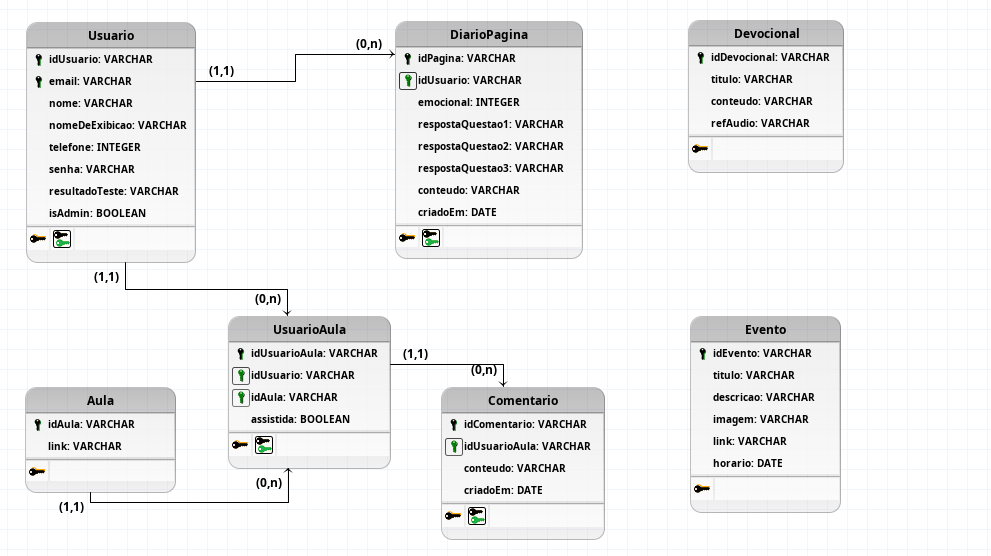
\includegraphics[width=1\linewidth]{conteudo//3 - ages II//conteudo//figures/soul-bd-logic}
  Fonte: \textit{Wiki} do projeto
  \label{fig:db-logic}
\end{figure}

Além das tabelas de usuários e postagens, foram criadas tabelas para os devocionais, vídeo aulas, comentários e eventos. A tabela de eventos foi criada para armazenar eventos que seriam exibidos no aplicativo, como encontros e palestras. Já a tabela de comentários teve o propósito de armazenar os comentários feitos pelos usuários nas vídeo aulas.

\subsection{Arquitetura Utilizada}
A estrutura arquitetural do projeto é baseada no design de interação entre componentes distintos. Uma parte do sistema atua como requisitante de serviços ou recursos (o \textit{frontend}, ou cliente), enquanto outra é responsável por processar essas solicitações e fornecer as respostas correspondentes (a API, ou servidor).

A API do projeto Soul Amada é executada em um container Docker hospedado em uma instância \ac{ec2} dentro de uma \ac{vpc} privada, com comunicação direta com o banco de dados da aplicação. O \textit{backend} utiliza o Supabase, uma solução escalável e autogerenciada, para armazenar os dados de forma eficiente.

Para o armazenamento de arquivos, um bucket do \ac{s3} foi integrado, simplificando o gerenciamento de dados pela API. Além disso, um API Gateway foi configurado para redirecionar chamadas para a instância EC2, garantindo acesso facilitado e organizado aos serviços da aplicação. É ilustrada esta arquitetura de \textit{cloud} na figura 17.

\begin{figure}[H]
  \centering
  \small
  \caption{Diagrama da arquitetura na nuvem do projeto Soul Amada}
  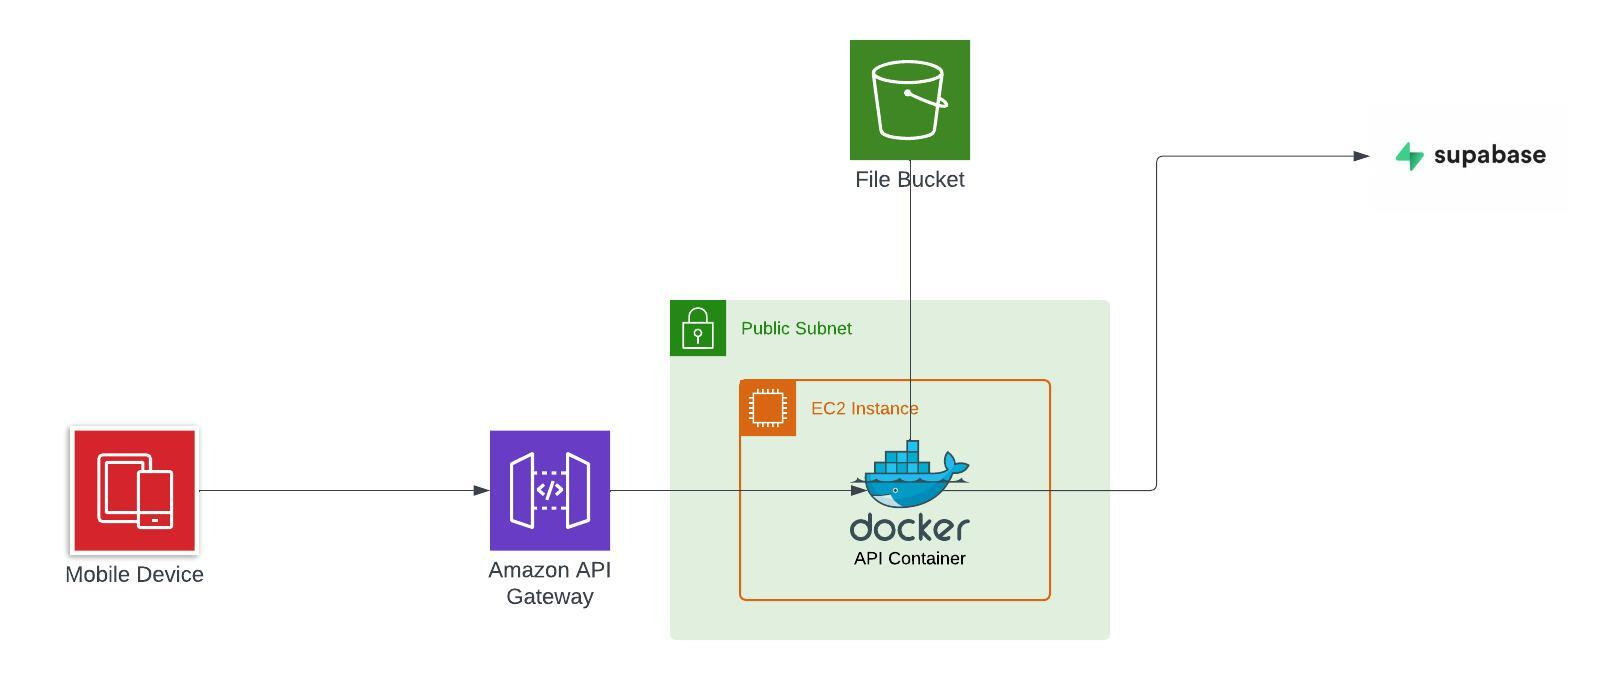
\includegraphics[width=1\linewidth]{conteudo//3 - ages II//conteudo//figures/infra.png}
  Fonte: \textit{Wiki} do projeto
  \label{fig:infra-api}
\end{figure}

Referente aos \textit{deploys}, o da API ocorre automaticamente após um commit na branch "main" do repositório \textit{backend}. Um \textit{runner} do GitLab é acionado na própria instância EC2, responsável por executar os testes e aplicar as migrações do \textit{Prisma} \ac{orm} no banco de dados do Supabase. Em seguida, o \textit{runner} realiza o build da imagem atualizada da API, finalizando qualquer container em execução previamente e iniciando um novo container com a imagem recém-criada, garantindo a atualização do serviço de forma contínua e eficiente.

O \textit{deploy} do front end também utiliza este mesmo \textit{runner} na EC2 para realizar  a criação da \ac{apk} e da \ac{ipa}. Este \textit{runner} enviará estes arquivos para uma pasta de releases no S3, onde o download das versões será disponibilizado. As figuras 18 e 19 ilustram o fluxo de \textit{deploy} do \textit{backend} e do \textit{frontend}, respectivamente.


\begin{figure}[H]
  \centering
  \small
  \caption{Diagrama da pipeline de \textit{deploy} da API do projeto Soul Amada}
  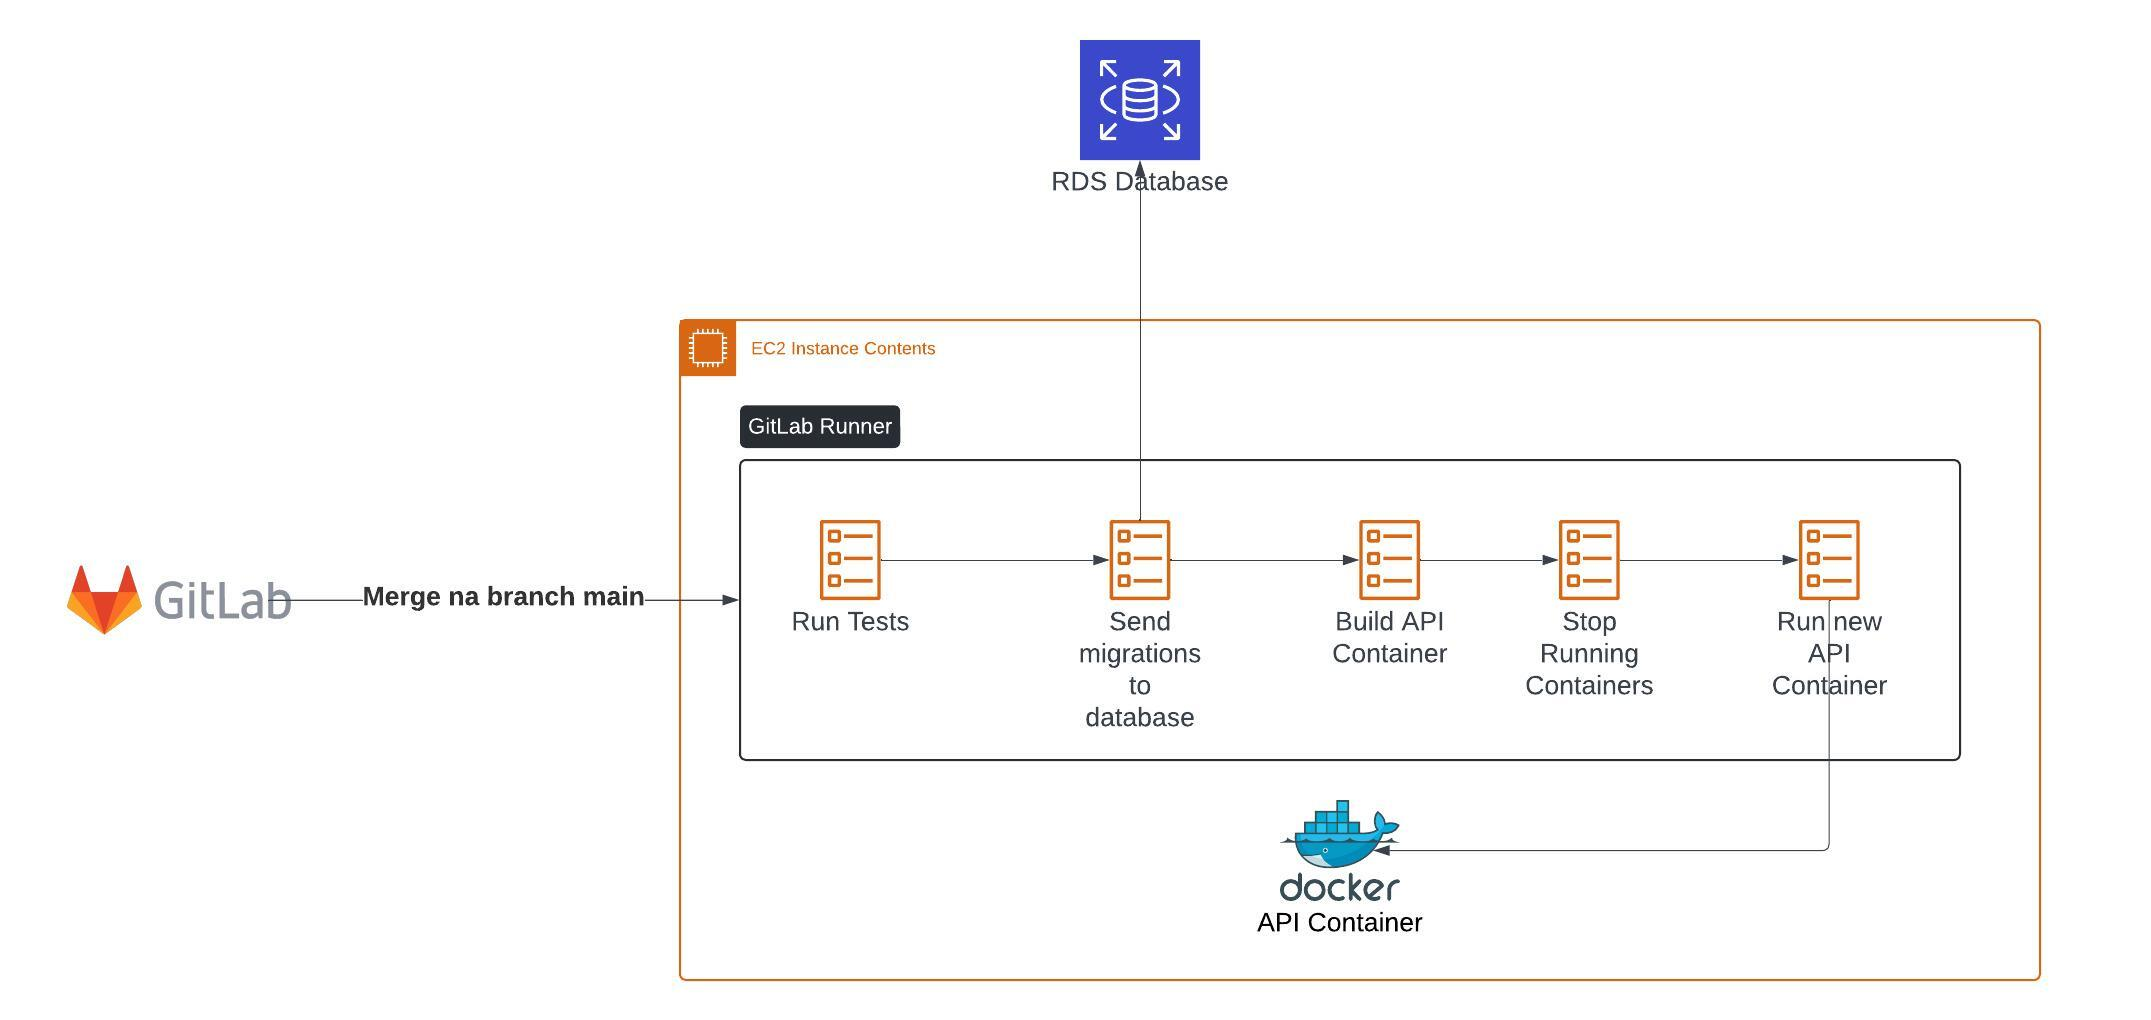
\includegraphics[width=1\linewidth]{conteudo//3 - ages II//conteudo//figures/infra-pipe.png}
  Fonte: \textit{Wiki} do projeto
  \label{fig:infra-api-deploy}
\end{figure}


\begin{figure}[H]
  \centering
  \small
  \caption{Diagrama da pipeline de \textit{deploy} do \textit{frontend} do projeto Soul Amada}
  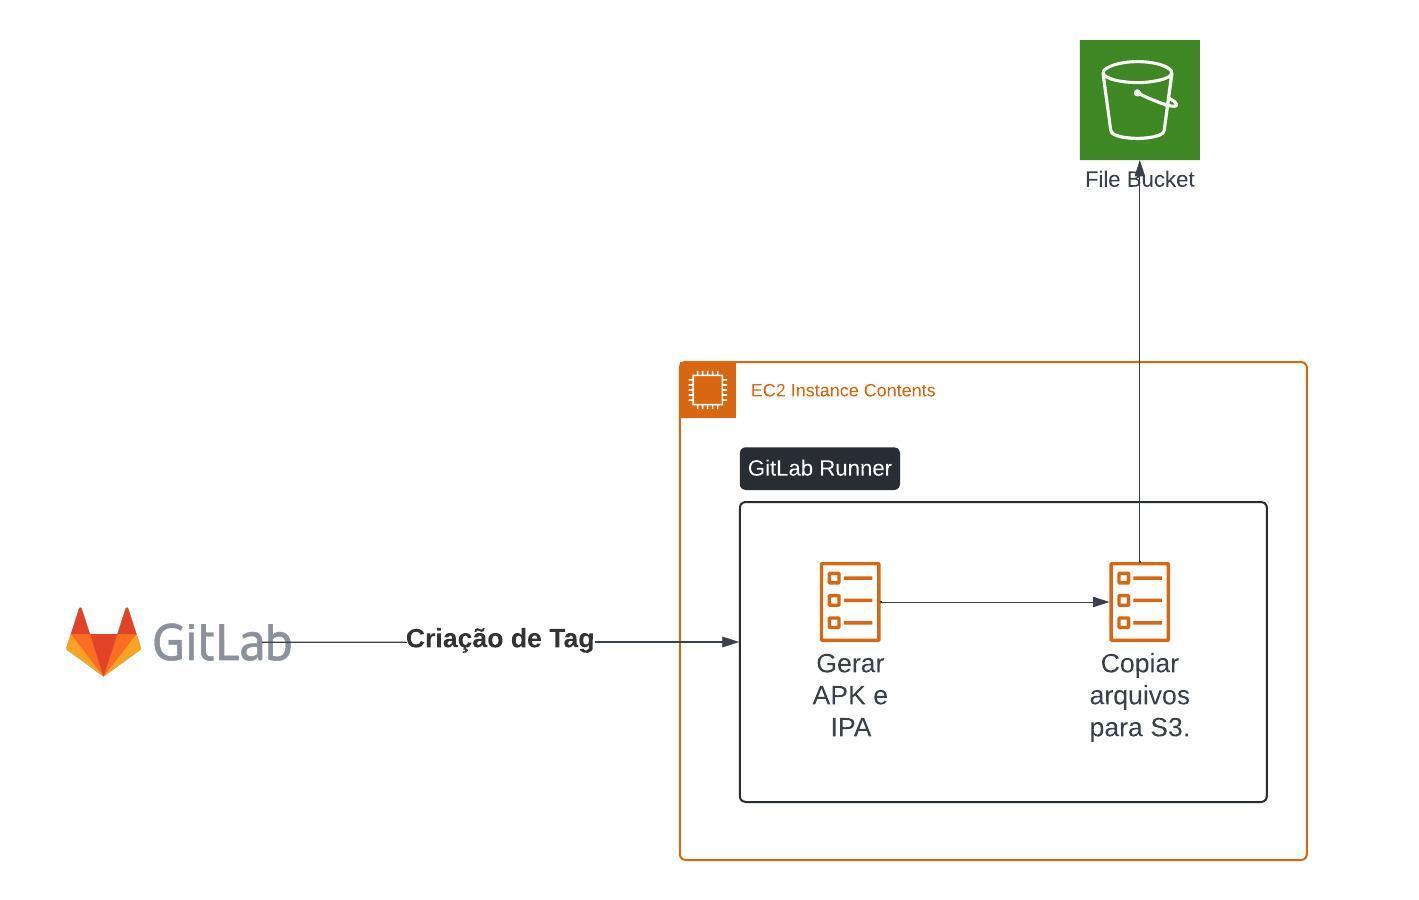
\includegraphics[width=1\linewidth]{conteudo//3 - ages II//conteudo//figures/infra-pipe-front.png}
  Fonte: \textit{Wiki} do projeto
  \label{fig:infra-front-deploy}
\end{figure}




\subsection{Protótipos das Telas Desenvolvidas}
Deverão ser apresentados os links da Wiki, com uma breve descrição.

\subsection{Tecnologias Utilizadas}

De uma maneira geral a tecnologia mais utilizada foi a linguagem TypeScript, tanto no \textit{frontend} quanto no \textit{backend} e diferenciando-se apenas nos \textit{frameworks} utilizados. No \textit{frontend} foi utilizado o React Native, enquanto no \textit{backend} foi utilizado o Nest.js. Além disso, o \ac{sgbd} utilizado foi o Supabase, que é um banco de dados PostgreSQL com uma camada de abstração para facilitar o uso.

Recursos da AWS também foram utilizados, como o EC2, S3 e API Gateway. O EC2 foi utilizado para hospedar a API, o S3 para armazenar arquivos e o API Gateway para redirecionar chamadas para a instância EC2.
